%%%%%%%%%%%%%%%
% English application CV
% Compile with XeLaTeX
\documentclass[a4paper,10pt]{article}

\usepackage[a4paper,left=1.18cm,right=1.18cm,top=0.68cm,bottom=0.72cm]{geometry}
\usepackage{graphicx}
\usepackage{enumitem}
\usepackage{tabularx}
\usepackage{hyperref}
\usepackage{xcolor}
\usepackage{fontspec}
\usepackage{setspace}
\usepackage[fixed]{fontawesome5}

\setmainfont[
  Path=/System/Library/Fonts/Supplemental/,
  UprightFont={Times New Roman.ttf},
  BoldFont={Times New Roman Bold.ttf},
  ItalicFont={Times New Roman Italic.ttf},
  BoldItalicFont={Times New Roman Bold Italic.ttf}
]{Times New Roman.ttf}
\setsansfont[
  Path=/System/Library/Fonts/Supplemental/,
  UprightFont={Times New Roman.ttf},
  BoldFont={Times New Roman Bold.ttf},
  ItalicFont={Times New Roman Italic.ttf},
  BoldItalicFont={Times New Roman Bold Italic.ttf}
]{Times New Roman.ttf}
\setmonofont[
  Path=/System/Library/Fonts/Supplemental/,
  UprightFont={Times New Roman.ttf},
  BoldFont={Times New Roman Bold.ttf},
  ItalicFont={Times New Roman Italic.ttf},
  BoldItalicFont={Times New Roman Bold Italic.ttf},
  Scale=0.96
]{Times New Roman.ttf}

\definecolor{rulegray}{HTML}{D8D2C8}
\definecolor{markerred}{HTML}{8A1538}
\definecolor{deepred}{HTML}{8A1538}
\definecolor{softgray}{HTML}{E6E0D6}
\definecolor{textgray}{HTML}{333333}

\setstretch{1.05}
\setlength{\parindent}{0pt}
\setlength{\parskip}{1.0pt}
\setlist[itemize]{leftmargin=1.15em,itemsep=0.7pt,topsep=0.7pt,parsep=0pt}
\hypersetup{hidelinks,colorlinks=false}
\pagestyle{empty}

\newcommand{\sectionhead}[1]{%
  \vspace{5.2pt}%
  \noindent{\fontsize{13.1}{14.1}\selectfont\bfseries #1}\par\vspace{0pt}%
  {\color{deepred}\rule{2.4em}{0.7pt}}{\color{rulegray}\rule{\dimexpr\textwidth-2.4em\relax}{0.45pt}}\par\vspace{2.0pt}%
}
\newcommand{\contacticon}[1]{\textcolor{deepred}{#1}\hspace{0.34em}}
\newcommand{\role}[1]{\textbf{\textcolor{textgray}{#1}}}
\newcommand{\dateright}[1]{\hfill{\footnotesize\textcolor{textgray}{#1}}}
\newcommand{\paperitem}[4]{%
  \noindent\makebox[1.0em][l]{\textcolor{markerred}{\footnotesize\faBookmark}}%
  \begin{minipage}[t]{\dimexpr\textwidth-8.0em\relax}\raggedright\textbf{#1}\end{minipage}%
  \makebox[7.0em][r]{\footnotesize\textcolor{textgray}{#2}}\par\vspace{-2pt}
  \hspace*{1.0em}\begin{minipage}[t]{\dimexpr\textwidth-1.0em\relax}
    #3\\[-1pt]
    {\small #4}
  \end{minipage}\par\vspace{2pt}
}

\begin{document}

\noindent\begin{minipage}[t]{0.775\textwidth}
  {\fontsize{17.2}{19.0}\selectfont\bfseries Cheng Chen}\\[0.2pt]
  {\fontsize{10.0}{11.5}\selectfont\textcolor{deepred}{Prospective PhD Applicant}}\\[0.2pt]
  {\fontsize{11.2}{12.8}\selectfont\bfseries Tongji University · Electrical Engineering}\\[3pt]
  {\fontsize{10.5}{12.0}\selectfont
  \begin{tabularx}{\linewidth}{@{}>{\raggedright\arraybackslash}X>{\raggedright\arraybackslash}X@{}}
    \contacticon{\faEnvelope}\href{mailto:2351445@tongji.edu.cn}{2351445@tongji.edu.cn} &
    \contacticon{\faEnvelope}\href{mailto:chenceason10@gmail.com}{chenceason10@gmail.com} \\
    \contacticon{\faGlobe}\href{https://ceasonen.github.io}{ceasonen.github.io} &
    \contacticon{\faGithub}\href{https://github.com/ceasonen}{github.com/ceasonen} \\
    \contacticon{\faUniversity}Major rank 3/87 &
    \contacticon{\faMapMarker}Shanghai, China
  \end{tabularx}}
\end{minipage}%
\hfill%
\begin{minipage}[t]{0.16\textwidth}
  \raggedleft
  \vspace{0.00cm}
  \setlength{\fboxsep}{0pt}\setlength{\fboxrule}{0.35pt}%
  \fcolorbox{softgray}{white}{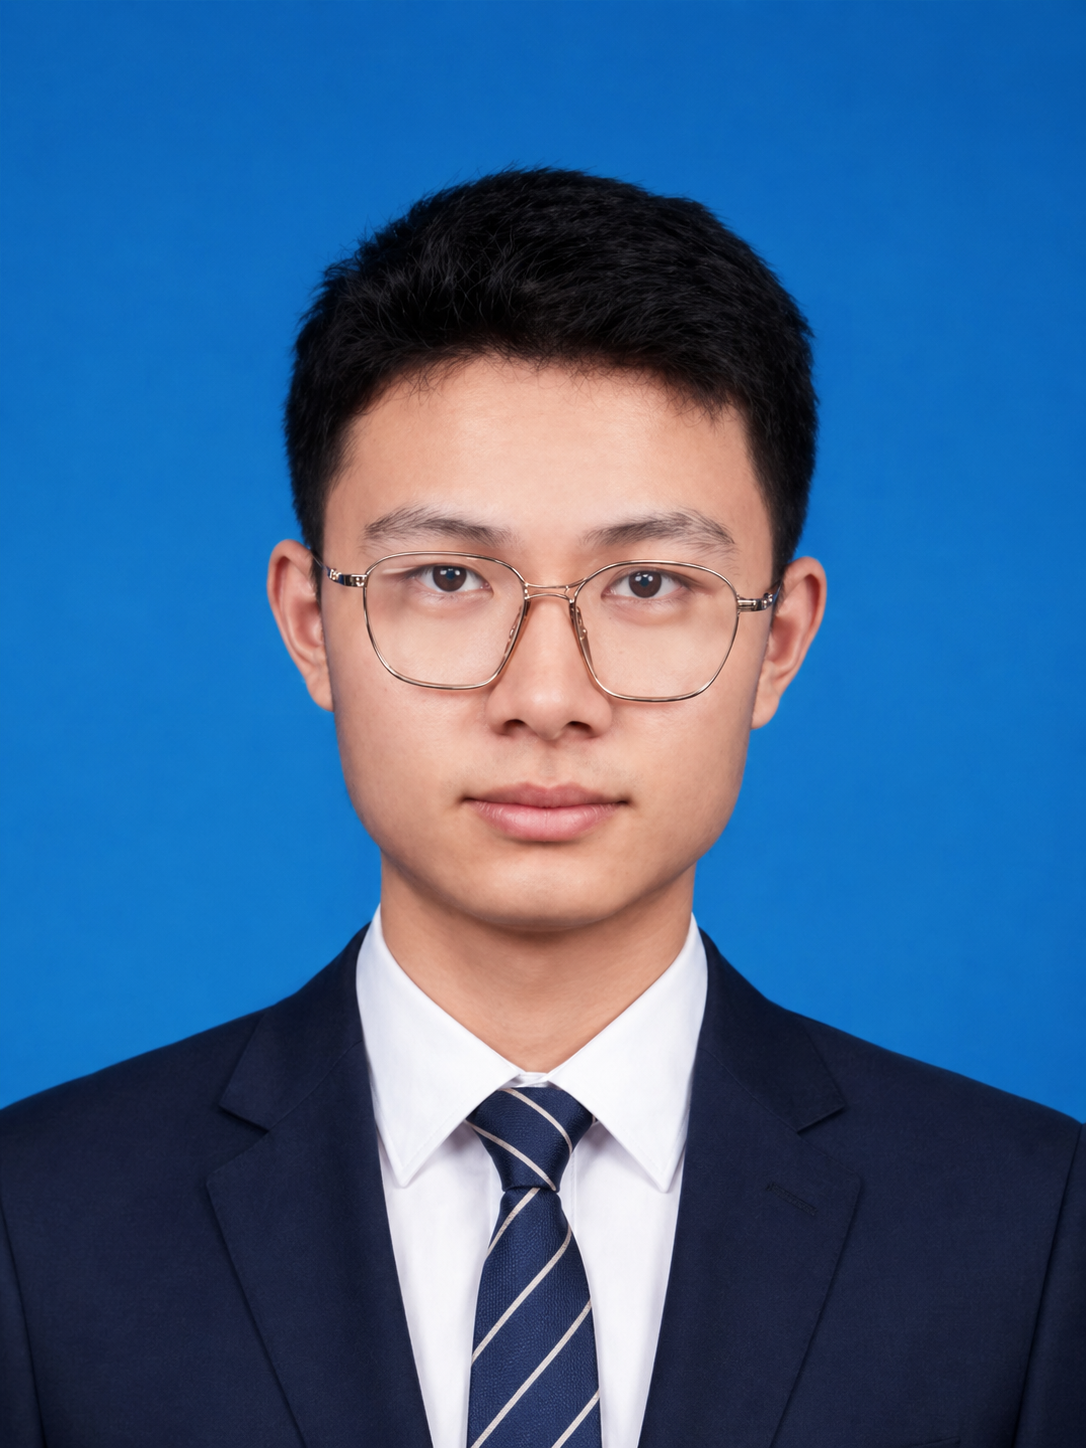
\includegraphics[width=2.18cm]{me.png}}
\end{minipage}\par\vspace{2pt}

\sectionhead{Summary}
\begin{itemize}
  \item EE undergrad at Tongji (rank \textbf{3/87}). Research on \textbf{multimodal AI} and \textbf{trustworthy AI}.
  \item Accepted papers at \textbf{IJCAI}, \textbf{IJCNN}, \textbf{ICANN}; submissions to \textbf{ACM MM} and \textbf{NeurIPS}.
\end{itemize}

\sectionhead{Education}
\textbf{B.Eng. in Electrical Engineering, Tongji University}, Shanghai \dateright{2023.09 -- Present}\\[-1pt]
Major rank: \textbf{3/87}; CET-6: \textbf{519}.

\sectionhead{Research}
\paperitem{OrthKD: Extracting Generalized Clinical Knowledge from Heterogeneous Teachers for Lightweight Deployment}{IJCAI 2026}
{\textbf{C. Chen}*, Y. Xu*, M. Cao. \role{Accepted; co-first; oral.}}
{Distill multiple clinical models into one small model without inheriting each teacher's bias.}

\paperitem{Open-Vocabulary Audio-Visual Event Localization}{ACM MM 2026}
{\textbf{C. Chen}* et al. \role{Under review; co-first. Initial score 4/4/4/4/3.}}
{Locate audio-visual events from any text query, with reliability-aware distillation.}

\paperitem{Enabling Visual Reasoning in Text-Only LLMs via Symbolic Scene Descriptions}{IJCNN 2026}
{W. Lei, M. Cao, C. Ye, Y. Xu, \textbf{C. Chen}. \role{Accepted; corresponding author.}}
{Describe scenes in symbols so text-only LLMs can reason about images.}

\paperitem{Beyond Relevance: Counter-Evidence Planning in a Controlled Budgeted RAG Testbed}{ICANN 2026}
{Y. Cai, Y. Xu, \textbf{C. Chen}. \role{Accepted; corresponding author.}}
{Plan retrieval under a fixed budget, including evidence that might disagree.}

\paperitem{Neural-Operator Risk Assessment for Deployable Risk Triage}{NeurIPS 2026}
{\textbf{C. Chen} et al. \role{Under review; first author.}}
{Flag risky neural-operator outputs in one forward pass.}

\sectionhead{Awards}
\begin{tabularx}{\textwidth}{@{}Xr@{}}
  National 2nd Prize, Global Campus AI Algorithm Elite Competition & 2025 \\
  National 3rd Prize, Embedded Chip \& System Design Competition & 2025 \\
\end{tabularx}

\sectionhead{Skills}
\begin{itemize}
  \item \role{Experiments:} PyTorch — training, baselines, ablations, and writing up what actually happened.
  \item \role{Writing:} English papers in LaTeX; first author, co-first, and corresponding author experience.
\end{itemize}

\end{document}
